
Aujourd'hui, la mammographie est la principale modalité d'imagerie pour le dépistage du cancer du sein et joue un rôle important dans son diagnostic. Les distorsions architecturales, les masses et les microcalcifications qui représentent un signe radiologique typique associé aux tissus cancéreux peuvent être visualisées au moyen d'imagerie par rayons X. Après une analyse détaillée, les résultats anormaux sont pris en charge pour une évaluation plus approfondie.

Le protocole standard en mammographie inclut la compression mammaire avant l'acquisition de l'image. Le sein est comprimé entre deux plaques jusqu'à l'obtention d'une épaisseur quasi-uniforme. L'aplatissement du sein améliore la qualité d'image et réduit la dose des photons ionisants absorbés par les tissus du sein. Cependant, l'inconfort et la douleur parfois provoquée par cette intervention peut dissuader les femmes de participer au programme de dépistage du cancer du sein par mammographie. Fleming et al. \citep{fleming_intermittent_2013} montrent que 15\% de femmes qui ont refusé le second rendez-vous pour une mammographie ont cité un premier examen désagréable ou douloureux.

Le confort du patient a pu être amélioré avec l'émergence de la mammographie numérique. Grâce à un détecteur plus performant, la qualité d'image et la quantité de dose ont pu être améliorées comparativement à la mammographie sur film. De plus, l'utilisation du Contrôle Automatique de l'Exposition ont permis d'estimer les paramètres d'acquisition fournissant la qualité d'image et la dose glandulaire moyenne optimales pour une épaisseur du sein et une glandularité données. Cela implique une possibilité de réduction de la compression du sein tout en respectant les normes cliniques sur la qualité de l'examen.

Dans ce contexte, le potentiel de d'imagerie par rayons X pourrait être contesté en développant des techniques alternatives de compression du sein. Les nouvelles techniques doivent tenir compte du confort du patient en plus d'une meilleure qualité d'image et d'une quantité de dose réduite. Cela peut impliquer une géométrie de pelotes différente ou des propriétés matérielles particulières ainsi qu'un positionnement distinct par rapport au sein.

L'objectif de cette thèse est de développer un environnement de simulation capable de caractériser l'impact du design de la pelote sur le confort du patient et ses répercussions sur la qualité de l'image et la quantité de dose en mammographie. Dans ce but, un modèle biomécanique du sein basé sur la théorie des éléments finis permettant d'estimer la déformation du sein sous compression a été développé. La géométrie du sein comprimé a été ensuite importée dans un environnement de simulation permettant de générer une image de mammographie syntactique et ainsi calculer la qualité d'image correspondante. 

Avant l'utilisation du modèle biomécanique dans le cadre de la compression du sein, sa capacité de simuler les déformations réelles des tissus doit être évaluée. L'imagerie par résonance magnétique (IRM) est une des seules modalités permettant d'imager le volume complet du sein ainsi que ses structures internes. Par conséquent, nous avons acquis des images RM de deux volontaires en trois positions différentes (sur le ventre, sur le dos et de côté,  Figure \ref{fig:donneespatient}).  Puisque les contraintes physiques de ces déformations peuvent être facilement reproduites dans un environnement de simulation, elles ont été utilisées pour le développement et l'évaluation de notre modèle biomécanique.     

\begin{figure}[!h]
\centering
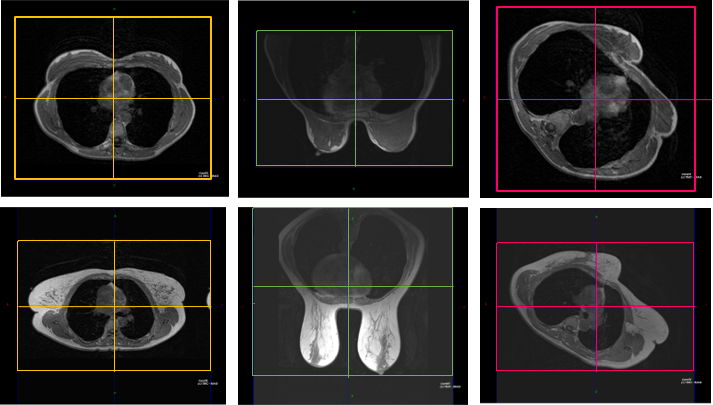
\includegraphics[width=0.9\textwidth,keepaspectratio]{figures/patientData.png} 
\caption{Les volumes IRM de deux voluntaires en trois configurations differente: première ligne - volontaire 1; deuxième ligne - volontaire 2}\label{fig:donneespatient}
\end{figure}


Les deux volontaires ont accepté de participer à une étude pilote approuvée par un comité d'éthique (étude pilote MammoBio MAP-VS). Les volontaires ont 59 et 58 ans et ont des tailles de sein différentes: coupe A (sujet 1) et coupe F (sujet 2) respectivement. Les volontaires ont été aussi demande de donner les informations de leurs dernier examen de mammographie comme la force appliquée et l'épaisseur du sein comprimée. Ces données serons utilisées comme référence lors de la simulations de la compression du sein. 
\begin{table}[!h]
\centering
\begin{tabular}{c|c|c||c|c|}
\cline{2-5}
&\multicolumn{2}{c||}{Subject 1}&\multicolumn{2}{c|}{Subject 2}\\
\cline{2-5}
& Right breast & Left breast & Right breast & Left breast\\
\cline{2-5}
\hline
\multicolumn{1}{|c||}{Force (N)}  & 21.9 &40.9 &94.8 & 56.6 \\
\hline
\multicolumn{1}{|c||}{ Breast thickness (mm)} & 47 & 42 & 50 & 49 \\
\hline

\end{tabular}
\caption{Compression force and breast thickness for both subjects for a cranio-caudal mammogram}\label{tab:forceandthichnessdata}
\end{table}

A cause d'un processus d'optimisation long est compliqué ainsi que des problèmes de convergence de la solution qui serront détaillées ultérieurement, les simulations des déformations du sein dues a la gravité (i.e. corps en position couché sur ventre, couché sur le dos et couche sur le côté) ont été calculée en utilisant juste le volume de la première volontaire. Au contraire, les déformations du sein dues a la compression entre deux plaques ont été calculées pour les deux volumes.

\subsection*{Modélisation biomechanique du sein}

Les images RM de la première volontaire en position couché sur le ventre ont été segmenté afin  d'extraire le volume de la cage thoracique (incluant le muscle pectorale) et le volume du sein . Ces deux volumes ont été utilisé pour générer le maillage d'éléments finis. Suite à une analyse de convergence du maillage, la taille des éléments finis permettant une bonne estimation des déformations avec un temps de calcul raisonnable  a été déterminée. La taille des éléments choisie varie entre $7mm$ et $10mm$.

Afin de modéliser le glissement des tissus adipeux sur le muscle pectorale une surface de contact a été créée en utilisant un modèle \textit{sans-séparation} proposé par l'environnement des simulations par éléments finis ANSYS. Des structures plus rigides ont été ajoutées pour faciliter la convergence de la solution en limitant le glissement des tissus mous du sein. Ceux-là ont été ajoutés en se basant sur la structure anatomique de la matrice de support du sein. La matrice de support est constituée de la fascia superficielle et la fascia profonde ainsi que de quatre ligaments suspenseurs: le ligament médial, le ligament inframammaire, le ligament latéral profond et le ligament cranial profond.  Dans notre modèle d'éléments finis, la fascia profonde a été modélisée par une couche d'éléments coque partageant les même nœuds que les éléments appartenant aux tissus en-dessous. La fascia superficielle et la peau ont été intégrées dans une seule couche d'éléments coque avec des propriétés mécaniques équivalentes à ce mélange. Seuls deux ligaments suspenseurs, le ligament médiale et le ligament inframammaire, ont été modélisés à l'aide des éléments de liaison.


Pour fournir un support rigide aux tissus du sein, des nœuds ont été définis sur la face postérieure du maillage représentant la cage thoracique.
Des conditions aux limites de Dirichlet supplémentaires ont été imposées sur les bords du maillage représentant le sein: les extrémités supérieure et inférieure de la couche du fascia profonde sont contraintes dans la direction Z; les extrémités supérieure et inférieure de la couche de peau sont contraintes dans la direction Y. Les bord latéraux du maillage de nouvelles structures ligamentaires sont incluses en utilisant des éléments de liaison avec un comportement de type câble.

Le modèle biomécanique du sein est composé de 5 composantes: le muscle, le sein, la peau, la fascia, et les ligaments. Chaque composante est définie par un type de tissu. A part les ligaments qui ont été modélisés en utilisant un matériel linéaire, tous les autres types de tissus on été modélisés en utilisant la fonction d'énergie de Neo-Hook. Les paramétrés constitutifs de ces modèles ont été optimisés tel que les estimations de la géométrie du sein dans la configuration couché sur le dos et couché sur le ventre soient le plus proche possible de la géométries du sein mesurés sur les images RM dans les configurations correspondantes. Dans ce but, la géométrie sans-contrainte du sein a été estimée en utilisant un algorithme basé sur le schéma de prédiction-correction itératif proposé par Carter T. \cite{carter_biomechanical_2009}. Cette méthode a été appliquée pour un ensemble exhaustif des propriétés mécaniques des tissus définis en utilisant le panel des valeurs existent dans la bibliographie. Les paramètres fournissant la meilleure correspondance entre les géométries du sein simulées et mesurées sont données par ($\lambda_{breast}^r=0.3 kPa$, $\lambda_{breast}^l=0.2 kPa$, $\lambda_{skin}=4 kPa$, $\lambda_{fascia}=120 kPa$).


La figure \ ref {fig: optimizationresults} montre les différences entre les géométries simulées et mesurées en configurations couchées sur le dos(à gauche) et couché sur le ventre (à droite). Chaque distance a été calculée sur un ensemble des nœuds distribuées a la surface de la peau en excluant les bras et les parties latérales due la cage thoracique.

\begin{figure}[!h]
\centering
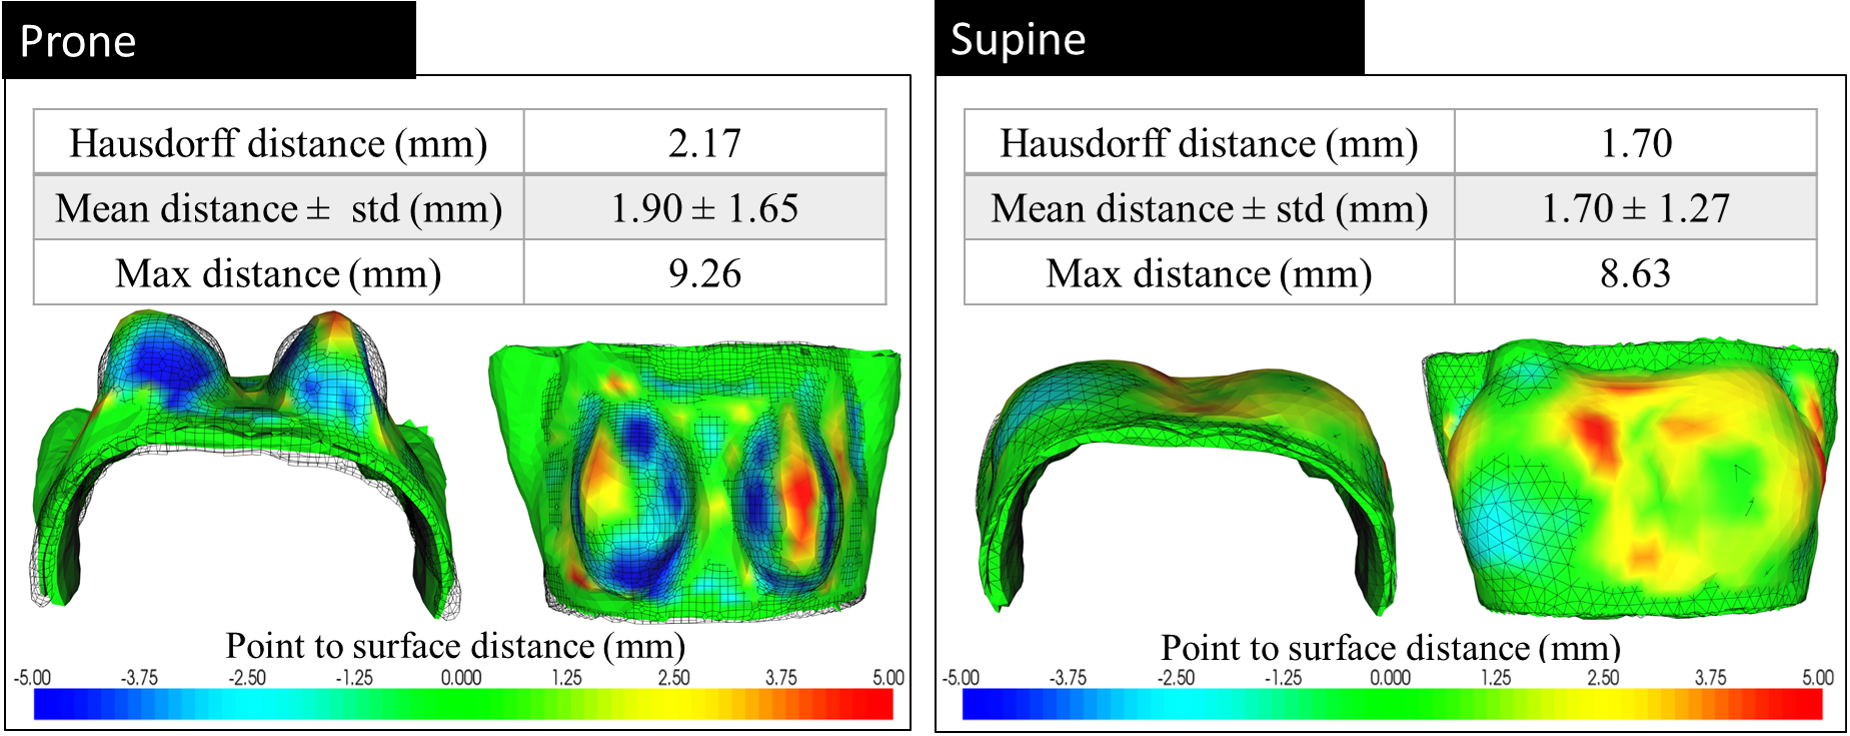
\includegraphics[width=\textwidth,keepaspectratio]{figures/optimizationresults.png} 
\caption{Difference  between estimated and measured data, in prone and supine configurations, obtained with optimal Young's moduli and stress-free geometry. }\label{fig:geometryoptimizationresults}
\end{figure}


La géométrie du sein est mieux estimée en décubitus dorsal, avec une distance de Hausdorff égale à 1,72 mm. Ceci est probablement dû à une meilleure représentation des conditions aux limites en configuration couchée, car cette configuration a été utilisée pour créer le maillage initial des éléments finis. La géométrie du sein en configuration couchée est également bien estimée, avec une distance de Hausdorff modifiée égale à 2,17 mm.

\begin{figure}[!h]
\centering
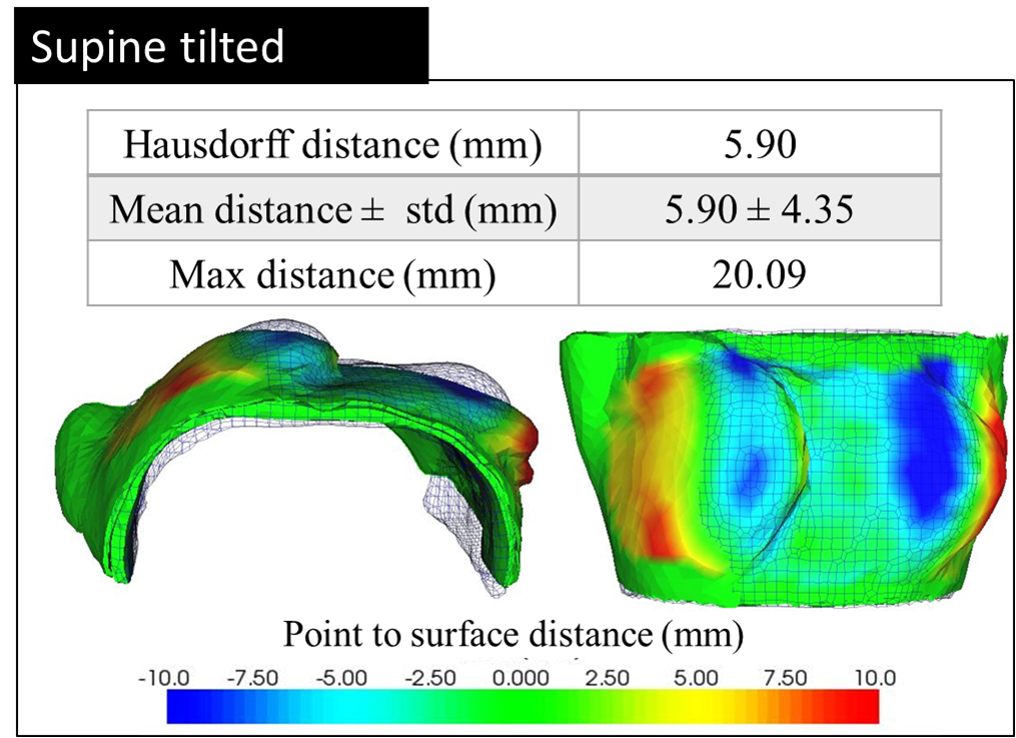
\includegraphics[width=0.6\textwidth,keepaspectratio]{figures/modelevaluation.png} 
\caption{Difference between estimated and measured breast geometries in supine tilted configuration.}\label{fig:modelevaluation}
\end{figure}

\begin{figure}[!h]
\centering
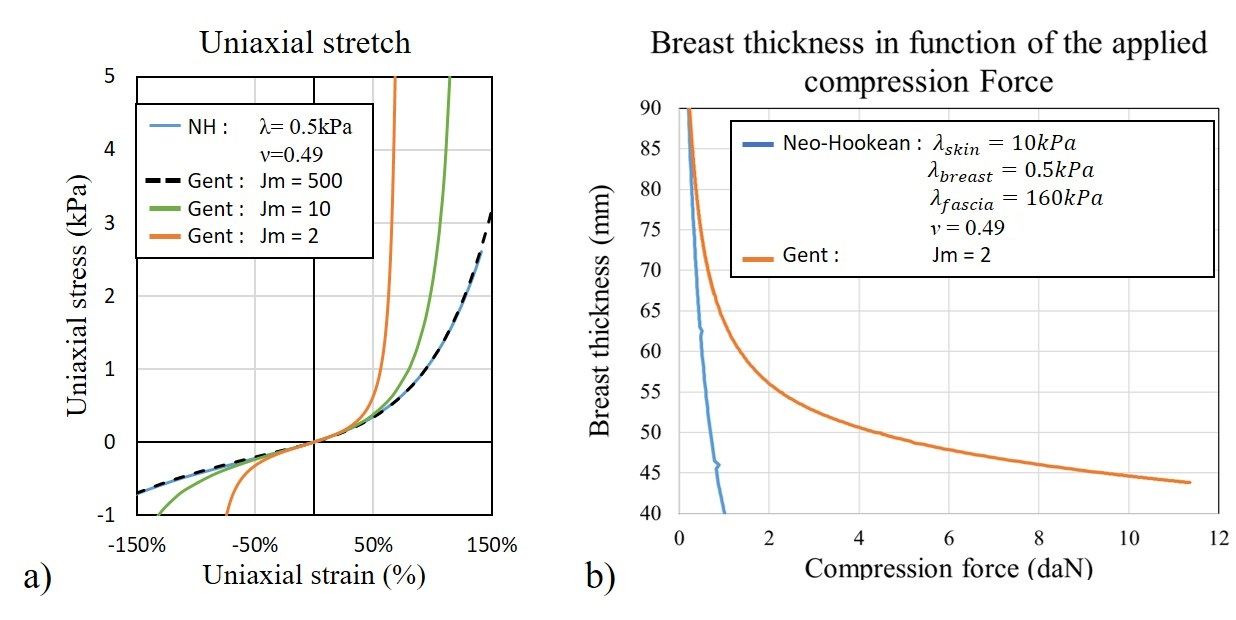
\includegraphics[width=1\textwidth,keepaspectratio]{figures/GentvsNeoStrain.jpg} 
\caption{a) Stress-strain relation for Neo-Hookean and Gent energy functions; b) Breast flattening curve as function of the applied force for a Gent energy function.}
\label{fig:GentvsNeoStrain}
\end{figure}


\begin{figure}[!h]
\centering
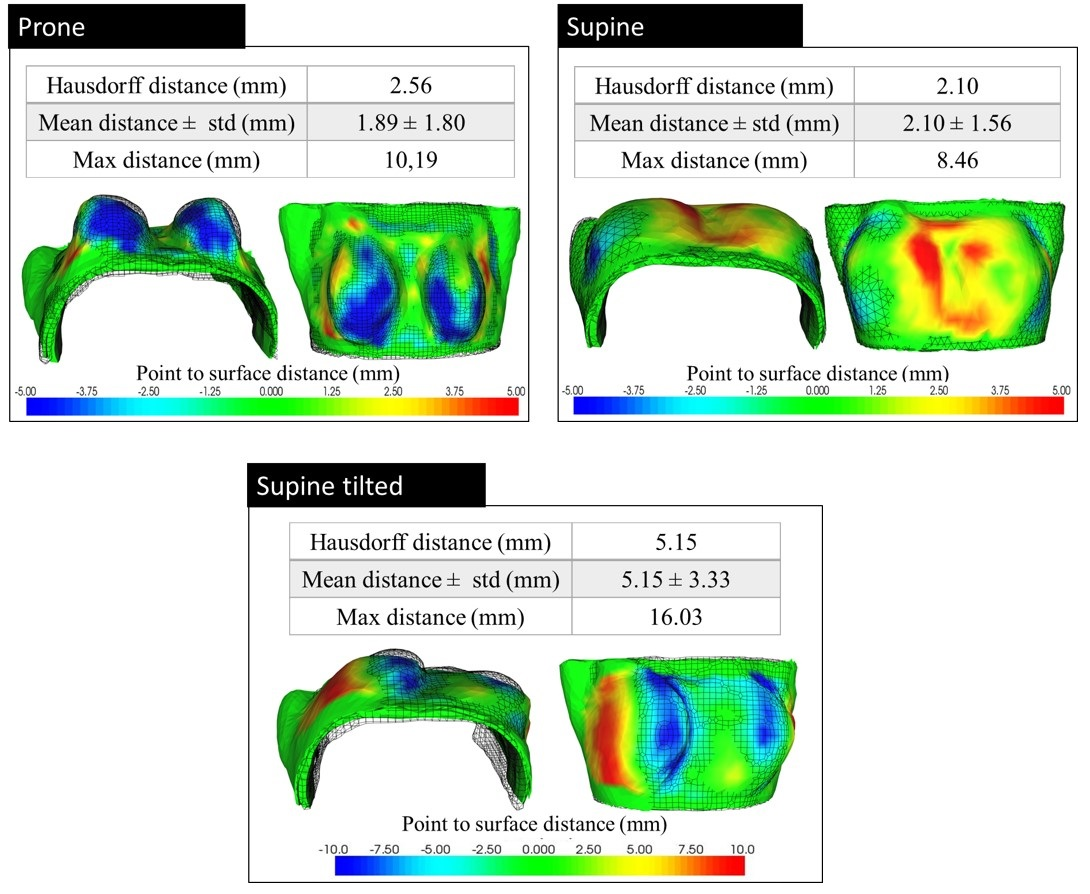
\includegraphics[width=\textwidth,keepaspectratio]{figures/modelevaluation_gent.jpg} 
\caption{Difference between estimated and measured data, in supine, prone and supine tilted configurations obtained with a Gent material model. }\label{fig:modelevaluation_gent}
\end{figure}